\documentclass{uncp-thesis}

% ----- CONFIGURACIÓN DE BIBLIOGRAFÍA -----
\addbibresource{src/bib/exported_items.bib}

% ----- DATOS DEL PLAN DE TESIS -----
\faculty{Ingeniería de Sistemas}
\thesistitle{Solución + Metodología + Problema + Contexto + Tiempo: SISTEMA DE INFORMACIÓN BASADO EN SCRUM/XP PARA LA TOMA DE DECISIONES EN XYZ-HYO, 2026}
\addauthor{Apellido Apellido\_1}{Nombre Nombre\_1}
% \addauthor{Apellido Apellido\_2}{Nombre Nombre\_2} % Quitar el comentario si se desea agregar más autores
\degree{Ingeniero de Sistemas}
\city{Huancayo}
\thesisyear{2026}

\begin{document}

% ----- 1. CARÁTULA -----
\makethesistitle

% ----- 2. PÁGINAS PRELIMINARES (Numeración romana) -----
\pagestyle{plain}
\pagenumbering{roman}
\setcounter{page}{2}

% ----- 4. CUERPO DEL PLAN DE TESIS (Numeración arábiga) -----
\pagestyle{fancy}
\pagenumbering{arabic}
\setcounter{page}{1}

\chapter{Línea de Investigación}

    Líneas de Investigación:

    \begin{figure}[H]
        \centering
    %\isPreprints{\centering}{} % Only used for preprints
        \caption{Líneas de Investigación. 
        \label{fig-lineas-investigacion}}    
        
        \includegraphics[width=15.0 cm]{src/files/Líneas_de_Investigación.pdf}

        \vspace{0.1cm}
        \small Elaborado a partir de ...
    \end{figure}

\chapter{Título}
    Título de la Investigación

\chapter{Asesor}
    Dra. ...

% -- PRIMER CAPÍTULO --
% PLANTEAMIENTO DEL PROBLEMA
\chapter{Planteamiento del Problema}
    El planteamiento del problema debe ser dividido en base a:

    \begin{itemize}
        \item \textbf{Descripción u contexto:} 3 u 4 líneas
        \item \textbf{Macrocontexto:} 1.5 páginas (Contexto más general - puedes verlo como el nivel mundial,  aunque no simboliza ello)
        \item \textbf{Mesocontexto:} 2 páginas (Contexto algo más específico - Podrías verlo como un contexto nacional u regional, aunque no simboliza ello)
        \item \textbf{Microcontexto:} 2.5 páginas (Contexto totalmente específico y exacto del tema - Podrías verlo como un contexto directo de tu tema, en la institución o demás)
        \item \textbf{Párrafo conclusivo del problema} (remembranza del planteamiento y una conclusión del mismo) => establece la naturaleza y la dimensión del problema, así como la importancia de la solución
    \end{itemize}

    \textbf{Párrafo de contexto del trabajo}. Lorem ipsum dolor sit amet consectetur adipisicing elit. Voluptate dolor sapiente accusamus vel tempore distinctio dicta architecto at beatae aliquam, cumque consequatur iure, aspernatur unde ratione a enim non molestiae voluptas nemo. Enim sed laudantium repellat odit eligendi quam facilis perspiciatis similique quo impedit praesentium eos error et corrupti quidem, aperiam consequuntur debitis libero tempora commodi aut voluptatum? Quasi numquam temporibus, tempore amet commodi tempora, mollitia hic esse molestias earum eligendi, sint rem suscipit! Quia est veritatis aspernatur nihil, eius consectetur tenetur quaerat, sunt quo numquam nesciunt ipsam iure reiciendis quisquam facilis totam obcaecati rem, culpa praesentium voluptates voluptatum sit. 

    \begin{figure}[H]
        \centering
        %\isPreprints{\centering}{} % Only used for preprints
        \caption{Una investigación nunca termina, solo se ve limitada por nosotroso
        \label{fig-contexto-investigacion}}    
                
        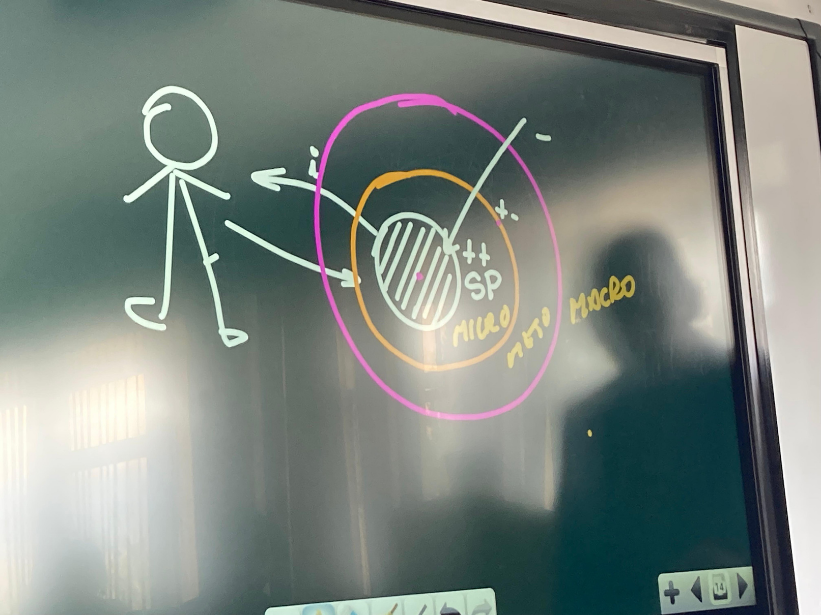
\includegraphics[width=6.0 cm]{src/imgs/nivel-contexto-investigacion.png}

        \vspace{0.1cm}
        % \small EN CASO DE SER BAJO ELABORACIÓN PROPIA, NO HACE FALTA AGREGAR LA NOTA
    \end{figure}
% --- RELLENAR ---
 % Los paréntesis en las secciones deben ser eliminados
\section{Primera sección (Macrocontexto)}
    \begin{sectext}
        Lorem ipsum dolor sit amet consectetur adipisicing elit. Voluptate dolor sapiente accusamus vel tempore distinctio dicta architecto at beatae aliquam, cumque consequatur iure, aspernatur unde ratione a enim non molestiae voluptas nemo. Enim sed laudantium repellat odit eligendi quam facilis perspiciatis similique quo impedit praesentium eos error et corrupti quidem, aperiam consequuntur debitis libero tempora commodi aut voluptatum? Quasi numquam temporibus, tempore amet commodi tempora, mollitia hic esse molestias earum eligendi, sint rem suscipit! Quia est veritatis aspernatur nihil, eius consectetur tenetur quaerat, sunt quo numquam nesciunt ipsam iure reiciendis quisquam facilis totam obcaecati rem, culpa praesentium voluptates voluptatum sit. 

        \begin{table}[!ht]
            % \centering
            \small % Un punto menos ayuda a la legibilidad en tablas densas
            \renewcommand{\arraystretch}{1} % Espacio equilibrado entre filas
            
            \caption{Atributos negativos frecuentemente asociados con las arquitecturas de pantallas volumétricas.}
            \label{tab:atributos-negativos-pantallas}

            % Usamos tabularx para que la tabla se ajuste exactamente al ancho de página
            \begin{tabularx}{\textwidth}{@{} >{\raggedright\arraybackslash\bfseries}p{3.5cm} X X @{}}
                \toprule
                \textbf{First Header} & \textbf{Second Header} & \textbf{Third Header} \\ 
                \midrule
                First Part & Second Part & Third Part \\
                \addlinespace[0.3cm]
                
                First Part & Second Part & Third Part \\
                \addlinespace[0.3cm]
                
                First Part & Second Part & Third Part \\
                \bottomrule
            \end{tabularx}
            
            \noindent{
                \footnotesize{
                    \textit{Nota.} Adaptado a partir de ...
                }
            }
    \end{table}

        Lorem ipsum dolor sit amet consectetur adipisicing elit. Voluptate dolor sapiente accusamus vel tempore distinctio dicta architecto at beatae aliquam, cumque consequatur iure, aspernatur unde ratione a enim non molestiae voluptas nemo. Enim sed laudantium repellat odit eligendi quam facilis perspiciatis similique quo impedit praesentium eos error et corrupti quidem, aperiam consequuntur debitis libero tempora commodi aut voluptatum? Quasi numquam temporibus, tempore amet commodi tempora, mollitia hic esse molestias earum eligendi, sint rem suscipit! Quia est veritatis aspernatur nihil, eius consectetur tenetur quaerat, sunt quo numquam nesciunt ipsam iure reiciendis quisquam facilis totam obcaecati rem, culpa praesentium voluptates voluptatum sit.
    
    \end{sectext}

\section{Segunda sección - Mesocontexto}
    \begin{sectext}
        \begin{figure}[H]
            \centering
        %\isPreprints{\centering}{} % Only used for preprints
            \caption{Logo UNCP. 
            \label{fig-uncp-logo}}    
            
            
\includegraphics[width=5.0 cm]{src/imgs/logo_uncp.png}

            \vspace{0.1cm}
            \small Elaborado a partir de ...
        \end{figure}

        Lorem ipsum dolor sit amet consectetur adipisicing elit. Voluptate dolor sapiente accusamus vel tempore distinctio dicta architecto at beatae aliquam, cumque consequatur iure, aspernatur unde ratione a enim non molestiae voluptas nemo. Enim sed laudantium repellat odit eligendi quam facilis perspiciatis similique quo impedit praesentium eos error et corrupti quidem, aperiam consequuntur debitis libero tempora commodi aut voluptatum? Quasi numquam temporibus, tempore amet commodi tempora, mollitia hic esse molestias earum eligendi, sint rem suscipit! Quia est veritatis aspernatur nihil, eius consectetur tenetur quaerat, sunt quo numquam nesciunt ipsam iure reiciendis quisquam facilis totam obcaecati rem, culpa praesentium voluptates voluptatum sit.
        \newline

    \end{sectext}


\section{Tercera sección - Microcontexto}
    \begin{sectext}
    Lorem ipsum dolor sit amet consectetur adipisicing elit. Voluptate dolor sapiente accusamus vel tempore distinctio dicta architecto at beatae aliquam, cumque consequatur iure, aspernatur unde ratione a enim non molestiae voluptas nemo. Enim sed laudantium repellat odit eligendi quam facilis perspiciatis similique quo impedit praesentium eos error et corrupti quidem, aperiam consequuntur debitis libero tempora commodi aut voluptatum? Quasi numquam temporibus, tempore amet commodi tempora, mollitia hic esse molestias earum eligendi, sint rem suscipit! Quia est veritatis aspernatur nihil, eius consectetur tenetur quaerat, sunt quo numquam nesciunt ipsam iure reiciendis quisquam facilis totam obcaecati rem, culpa praesentium voluptates voluptatum sit.
    \newline

    \end{sectext}


\textbf{Párrafo conclusivo del planteamiento del problema.} Lorem ipsum dolor sit amet consectetur adipisicing elit. Voluptate dolor sapiente accusamus vel tempore distinctio dicta architecto at beatae aliquam, cumque consequatur iure, aspernatur unde ratione a enim non molestiae voluptas nemo. Enim sed laudantium repellat odit eligendi quam facilis perspiciatis similique quo impedit praesentium eos error et corrupti quidem, aperiam consequuntur debitis libero tempora commodi aut voluptatum? Quasi numquam temporibus, tempore amet commodi tempora, mollitia hic esse molestias earum eligendi, sint rem suscipit! Quia est veritatis aspernatur nihil, eius consectetur tenetur quaerat, sunt quo numquam nesciunt ipsam iure reiciendis quisquam facilis totam obcaecati rem, culpa praesentium voluptates voluptatum sit.


% -- SEGUNDO CAPÍTULO --
% FORMULACIÓN DEL PROBLEMA
\chapter{Formulación del Problema}

        \begin{table}[!ht]
            % \centering
            \small % Un punto menos ayuda a la legibilidad en tablas densas
            \renewcommand{\arraystretch}{1} % Espacio equilibrado entre filas
            
            \caption{Simbologia utilizada para los problemas }
            \label{tab:atributos-negativos-pantallas}

            % Usamos tabularx para que la tabla se ajuste exactamente al ancho de página
            \begin{tabularx}{\textwidth}{@{} >{\raggedright\arraybackslash\bfseries}p{2.0cm} X @{}}
                \toprule
                \textbf{Símbolo} & \textbf{Significado} \\ 
                \midrule
                VD & Variable Dependiente \\
                \addlinespace[0.3cm]
                
                VI & Variable Independiente \\
                \addlinespace[0.3cm]
                                
                M & Metodología \\
                \addlinespace[0.3cm]

                C & Contexto \\
                \addlinespace[0.3cm]
                
                T & Tiempo \\
                \addlinespace[0.3cm]

                f & función (matemática) \\
                \bottomrule
            \end{tabularx}
            
            \noindent{
                \footnotesize{
                    \textit{Nota.} Adaptado a partir de ...
                }
            }
    \end{table}

\section{Problema General}
    \begin{sectext}
        ¿Cómo influye la VI en la VD en el C y T establecido?

        ¿Qué relación existe entre la implementación de VI + M y la VD en C y T?

        ¿De qué modo la VI + M afecta  a la VD en el C y T establecido?

        \textbf{¿Cómo influye la implementación de un sistema de información basado en SCRUM/XP en la toma de decisiones de en la empresa XYZ-Hyo - 2026?}
    \end{sectext}

\section{Problemas Específicos}
    \begin{sectext}
        \textbf{2 o 3 a lo máximo}

        \begin{itemize}
            \item ¿Cómo influye la disponibilidad de  información en la toma de decisiones en la empresa xyz -hyo, 2026

            \item ¿Cómo influye la calidad de información en la toma de decisiones en la empresa xyz-hyo, 2026?
        \end{itemize}
    \end{sectext}

% -- TERCER CAPÍTULO --
% OBJETIVOS DE LA INVESTIGACIÓN
\chapter{Objetivos de la Investigación}
\section{Objetivo General}
    \begin{sectext}
            Determinar la influencia de la VI en la VD en el C y T

            \textbf{Determinar la influencia de la implementación de un sistema de información basado en scrum/xp en la toma de decisiones en el contexto y tiempo establecidos.}
    \end{sectext}

\section{Objetivos Específicos}
    \begin{sectext}
        \textbf{Debe ser la misma cantidad que problemas}
            \begin{itemize}
                \item Lorem ipsum dolor sit amet consectetur adipisicing elit. Voluptate dolor sapiente accusamus vel tempore distinctio.

                \item Lorem ipsum dolor sit amet consectetur adipisicing elit. Voluptate dolor sapiente accusamus vel tempore distinctio dicta.
            \end{itemize}
    \end{sectext}

% -- CUARTO CAPÍTULO --
% MARCO DE REFERENCIA
\chapter{Marco de Referencia}

Se define como el basamento teórico y experimental. Este ayuda a entender mejor el problema, la metodología y la solución

\section{Antecedentes}
    \begin{sectext}
        Los antecedentes pueden desprenderse en 2 tipos:

        \begin{itemize}
            \item \textbf{Antecedentes del problema:} ¿Desde cuándo está presente tu problema?
            \item \textbf{Antecedentes de la investigación:} ¿Quiénes otros han estudiado ese problema?
        \end{itemize}

        % \newline 
        
        En la sección de antecedentes de las tesis nos referimos a los antecedentes de investigación. (Otros trabajos que ya han sido realizados). Estos tienen relación con el tema: Variables dependiente, independiente u la metodología.

        \begin{figure}[H]
            \centering
            %\isPreprints{\centering}{} % Only used for preprints
            \caption{Cantidad de Antecedentes necesarios. 
            \label{fig-cantidad-antecedentes}}    
                
            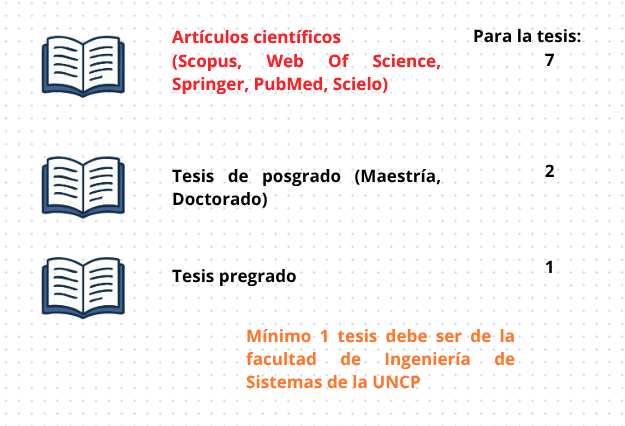
\includegraphics[width=10.0 cm]{src/imgs/cant-antecedentes.png}

            \vspace{0.1cm}
            \small Elaborado a partir de ...
        \end{figure}

        \begin{figure}[H]
            \centering
            %\isPreprints{\centering}{} % Only used for preprints
            \caption{Estructura de redacción de los antecedentes.
            \label{fig-estructura-antecedentes}}    
                
            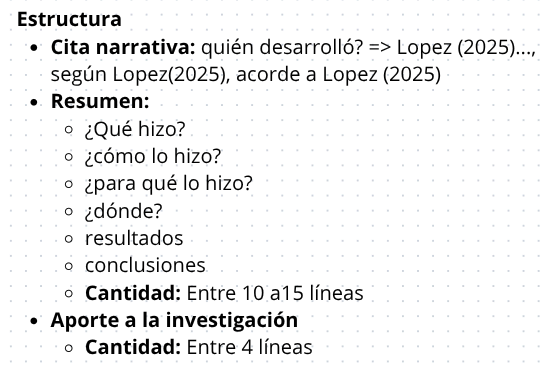
\includegraphics[width=10.0 cm]{src/imgs/estructura-antecedentes.png}

            \vspace{0.1cm}
            \small Elaborado a partir de ...
        \end{figure}

        \textcite{arensmeyer_system_2024}, describieron un novedoso sistema de planificación quirúrgica tridimensional en tiempo real basado en realidad mixta mediante el uso de un visor con tecnología de transmisión de video (video pass-through) y el renderizado volumétrico de datos de tomografía computarizada (TC). La investigación tuvo como finalidad mejorar la evaluación preprocedural y la planificación de tratamientos personalizados en cirugías complejas de la cavidad torácica, minimizando la necesidad de guías basadas en radiación intraoperatoria. Para validar el concepto, los autores aplicaron el sistema clínico en el Hospital Universitario de Bonn (Alemania), proyectando y alineando hologramas anatómicos interactivos sobre los cuerpos de tres pacientes oncológicos masculinos atendidos entre 2022 y 2023. Como principales resultados, los cirujanos lograron identificar con precisión las regiones de interés y distinguir la relación geométrica entre las lesiones y las estructuras blandas u óseas adyacentes utilizando herramientas de manipulación de imagen e integración de sensores LiDAR. Los autores concluyeron que el uso de superposiciones holográficas en entornos de realidad extendida resulta altamente prometedor para optimizar el abordaje de operaciones torácicas complejas o menos estandarizadas, proporcionando una perspectiva quirúrgica superior en comparación con las imágenes bidimensionales convencionales. El trabajo de \textcite{arensmeyer_system_2024} resalta el problema identificado por la presente investigación, aseverando que la poca utilización de las imágenes reconstruidas en 3D para la planificación quirúrgica de cirugías torácicas, los cuales al ser combinados con métodos inmercivos como la realidad Virtual u Mixta mejoran la precisión en la planificación. \newline
        
        \textcite{bakhuis_essential_2023} investigaron el valor clínico añadido de la tecnología de realidad virtual (RV) en el planeamiento preoperatorio de segmentectomías pulmonares. La investigación tuvo como finalidad evaluar la cantidad de modificaciones críticas en los planes quirúrgicos tradicionales y analizar la planificación preoperatoria ante una mejor perspectiva espacial de la anatomía broncovascular del paciente. El estudio se realizó con un equipo de tres cirujanos y un residente del Centro Médico de la Universidad de Erasmus en Rotterdam (Países Bajos); por su parte, se analizaron los resultados de 50 pacientes programados para resección segmental sublobar entre junio de 2020 y septiembre de 2021. El desarrollo metodologógico constó del procesamiento de las tomografías computarizadas (TC) convencionales mediante inteligencia artificial con la plataforma PulmoVR para realizar segmentaciones automáticas de los bordes pulmonares y vasos anatómicos. Como principales resultados, la visualización inmersiva en 3D provocó que los cirujanos modificaran el plan quirúrgico original en el 52\% de los casos (debido a localizaciones tumorales erróneas o variantes anatómicas ocultas), logrando una tasa de éxito de resección radical confirmada del 98\%. Los autores concluyeron que la integración de la realidad virtual preoperatoria proporciona una comprensión anatómica superior y personalizada, permitiendo realizar cirugías con mayor preservación de tejido pulmonar sano sin comprometer la radicalidad oncológica. El trabajo de \textcite{bakhuis_essential_2023} responde directamente a la problemática establecida por el presente trabajo respecto a la limitada imagen mental que los cirujanos son capaces de percibir respecto a la patología y anatomía del paciente solo mediante el uso de imágenes médicas en el marco bidimensional. \newline
    \end{sectext}
    

\section{Marco Teórico}
    \begin{sectext}
        Define hasta qué punto se enmarca la investigación.

        Como recomendación, no debes poner más conceptos de los que usarás. Ya que de lo contrario se custionará el: ¿Y dónde utilizó tal u tal concepto?

        Aquí de cierta manera se delimita el alcance. Míralo como los márgenes de un estadio de fútbol.

        \subsection{Concepto como subsección 1}
            \begin{subsectext}
                Lorem ipsum dolor sit amet consectetur adipisicing elit. Voluptate dolor sapiente accusamus vel tempore distinctio dicta architecto at beatae aliquam, cumque consequatur iure, aspernatur unde ratione a enim non molestiae voluptas nemo. Enim sed laudantium repellat odit eligendi quam facilis perspiciatis similique quo impedit praesentium eos error et corrupti quidem, aperiam consequuntur debitis libero tempora commodi aut voluptatum? Quasi numquam temporibus, tempore amet commodi tempora, mollitia hic esse molestias earum eligendi, sint rem suscipit! Quia est veritatis aspernatur nihil, eius consectetur tenetur quaerat, sunt quo numquam nesciunt ipsam iure reiciendis quisquam facilis totam obcaecati rem, culpa praesentium voluptates voluptatum sit. 

                \begin{itemize}
                    \item \textbf{Item 1}\newline
                    Lorem ipsum dolor sit amet consectetur adipisicing elit. Voluptate dolor sapiente accusamus vel tempore distinctio dicta architecto at beatae aliquam, cumque consequatur iure, aspernatur unde ratione a enim non molestiae voluptas nemo. 

                    \item \textbf{Item 2}\newline
                    Lorem ipsum dolor sit amet consectetur adipisicing elit. Voluptate dolor sapiente accusamus vel tempore distinctio dicta architecto at beatae aliquam, cumque consequatur iure, aspernatur unde ratione a enim non molestiae voluptas nemo.
                \end{itemize}
            \end{subsectext}

        \subsection{Concepto como subsección 2}
            \begin{subsectext}
                Lorem ipsum dolor sit amet consectetur adipisicing elit. Voluptate dolor sapiente accusamus vel tempore distinctio dicta architecto at beatae aliquam, cumque consequatur iure, aspernatur unde ratione a enim non molestiae voluptas nemo. Enim sed laudantium repellat odit eligendi quam facilis perspiciatis similique quo impedit praesentium eos error et corrupti quidem, aperiam consequuntur debitis libero tempora commodi aut voluptatum? Quasi numquam temporibus, tempore amet commodi tempora, mollitia hic esse molestias earum eligendi, sint rem suscipit! Quia est veritatis aspernatur nihil, eius consectetur tenetur quaerat, sunt quo numquam nesciunt ipsam iure reiciendis quisquam facilis totam obcaecati rem, culpa praesentium voluptates voluptatum sit. 

                \begin{itemize}
                    \item \textbf{Item 1}\newline
                    Lorem ipsum dolor sit amet consectetur adipisicing elit. Voluptate dolor sapiente accusamus vel tempore distinctio dicta architecto at beatae aliquam, cumque consequatur iure, aspernatur unde ratione a enim non molestiae voluptas nemo. 

                    \item \textbf{Item 2}\newline
                    Lorem ipsum dolor sit amet consectetur adipisicing elit. Voluptate dolor sapiente accusamus vel tempore distinctio dicta architecto at beatae aliquam, cumque consequatur iure, aspernatur unde ratione a enim non molestiae voluptas nemo.
                \end{itemize}

            \end{subsectext}
    \end{sectext}

\section{Modelo Aplicativo}
    \begin{sectext}
        Delimita el paso del modelo teórico al modelo aplicativo (de la teoría a la realidad)

        Flujograma desde el cual el tesista lleva toda la teoría a la práctica. Esto a través de una serie de pasos estructurados.

        \begin{figure}[H]
            \centering
            %\isPreprints{\centering}{} % Only used for preprints
            \caption{Estructura del modelo aplicativo.
            \label{fig-estructura-antecedentes}}    
                
            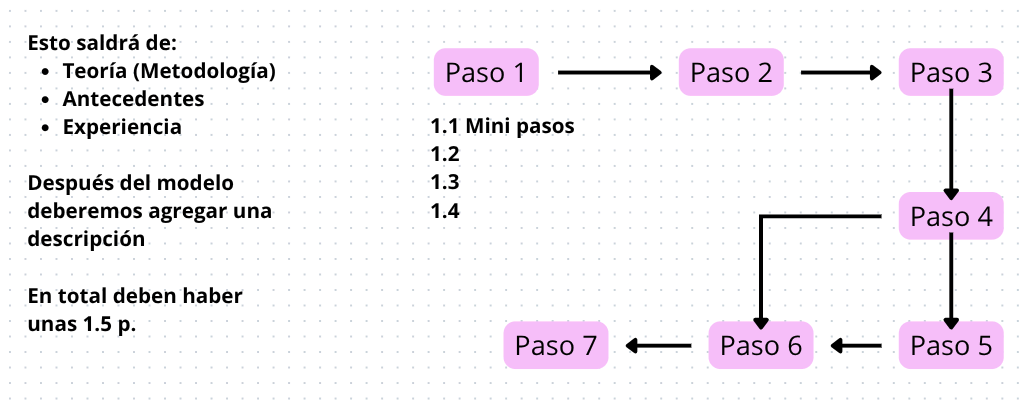
\includegraphics[width=10.0 cm]{src/imgs/modelo-aplicativo.png}

            \vspace{0.1cm}
            % \small EN CASO DE SER BAJO ELABORACIÓN PROPIA, NO HACE FALTA AGREGAR LA NOTA
        \end{figure}

    \end{sectext}

\section{Marco Conceptual}
    \begin{sectext}
        Es un glosario u diccionario en el cual incluimos los términos que necesitamos definir, pero que no son tan relevantes como para considerar en el marco teórico. De preferencia siempre usar citas parentéticas.

        Debemos considerar entre 15 a 20 términos. y cada definición debe tener de entre 2 a 3 líneas. Los términos no deben estar enumerados, pero sí ordenados alfabéticamente.

        \begin{itemize}
        \item \textbf{Conflicto de Vergencia-Acomodación (VAC)}: Contradicción fisiológica que causa fatiga visual cuando los ojos convergen en un objeto 3D virtual pero deben enfocar físicamente (acomodación) a la distancia fija de una pantalla 2D convencional \parencite{blundell_uncertain_2017}.

        \item \textbf{Pantallas de volumen barrido (Swept-volume)}: Dispositivos volumétricos que crean el espacio de visualización mediante el movimiento mecánico rápido y cíclico (ya sea rotacional o de traslación) de una superficie de proyección \parencite{blundell_classification_2002}.
        
        \item \textbf{Technology Readiness Level (TRL)}: Escala de nueve niveles creada inicialmente por la NASA para evaluar la madurez, el riesgo y el avance de una nueva tecnología desde su concepción hasta su despliegue operativo \parencite{salazar_zegarra_taxonomitecnicas_2022}.

        \item \textbf{Vóxel}: Es el equivalente tridimensional de un píxel; consiste en una región o elemento de volumen localizado que emite, refleja o absorbe la luz para conformar una imagen gráfica sólida en el espacio \parencite{blundell_classification_2002}.
        \end{itemize}
    \end{sectext}


% -- QUINTO CAPÍTULO --
% JUSTIFICACIÓN
\chapter{Justificación}
Realizar la justificación de la investigación para una tesis debe realizarse desde 5 perspectivas:

\begin{itemize}
    \item \textbf{Justificación Teórica:} Validar, utilizar, cuestionar (Valida teoría)
    \item \textbf{Justificación Práctica:} Hablar de (Resuelve el problema)
    \item \textbf{Justificación Metodológica:} Recrear (Utilizar una metdología existente, llevarlo a otro lugar y ajustarlo u adaptarlo a las necesidades de ese nuevo entorno) Replicar (Copiar y pegar el modelo a otra zona sin considerar el contexto). Presenta a la comunidad académica un modelo aplicativo que es una forma de resolver problemas de tales u cuáles naturalezas, el mismo que puede ser recreado en otras investigaciones.
    \item \textbf{Justificación Social:} Tiene que estar enmarcado dentro de las ODS, Responsabilidad Social Univesitaria y los Ejes estrátegicos del plan nacional al 2050. (Genera una impacto en la organización u la empresa)
    \item \textbf{Justificación Económica:} Impacto de nuestra investigación sobre la competitividad, economía de la organización. No se necesario que sea numérico; En términos generales debemos explicar que a través de nuestra tesis se logrará la estabilidad de la organización, la competititvidad de la empresa, se va a asegurar las sostenibilidad en el etiempo de la empresa en el sector u negocio en el cual estamos trabajando.
\end{itemize}

Unas 6 líneas por cada justificación es lo ideal. Las siguientes secciones incluyen un inicio de la justificación, esto es un ejemplo de cómo realicé la justificación de mi trabajo, pero cada trabajo de tesis es especial y único.

\section{Justificación Teórica}
    \begin{sectext}
        La presente investigación se consolida al establecer la base del mismo en un conjunto de teorías en distintos ámbitos de conocimiento;...
    \end{sectext}

\section{Justificación Metodológica}
    \begin{sectext}
        La presente investigación se enmarca al uso de 2 métodos consolidados en el ámbito de la creación e invención tecnológica en materia de hardware y software...
    \end{sectext}

\section{Justificación Práctica}
    \begin{sectext}
        La presente investigación se centra en la superación de la carente...
    \end{sectext}

\section{Justificación Social}
    \begin{sectext}
        La presente investigación enmarca su desarrollo sobre los Objetivos de Desarrollo Sostenible 3 (Salud y Bienestar) y 9 (Industria, innovación e infraestructuras) debido a sus implicancias en el ámbito médico por medio del ámbito ingenieril. Por su parte, respecto a la Responsabilidad Social Universitaria, la investigación abarca el área de Intervención Tecnológica debido a la disposición de la investigación a proponer y ejecutar tecnologías en favor de problemas sociales de la comunidad. A su vez, respecto al Plan Estatrégico de Desarrollo Nacional al 2050, la investigación toma especial énfasis en el ON3. Competitividad e Innovación, siendo el OE 3.5 Elevar la capacidad científica y de innovación tecnológica del país el objetivo al cual la investigación se alinea con mayor relevancia.
    \end{sectext}

\section{Justificación Económica}
    \begin{sectext}
        La presente investigación busca mejorar la capacidad de análisis del...
    \end{sectext}

% -- SEXTO CAPÍTULO --
% HIPÓTESIS
\chapter{Hipótesis}
La hipótesis es la respuesta al problema de la investigación. La hipótesis, al igual que el problema y los objetivos se describen en tiempo presente. Siempre debemos intentar hacer que las relaciones sean positivas (Directamente), no negativas (Inversamente)

    \begin{figure}[H]
        \centering
        %\isPreprints{\centering}{} % Only used for preprints
        \caption{Hipótesis
        \label{fig-modelo-hipótesis}}    
                
        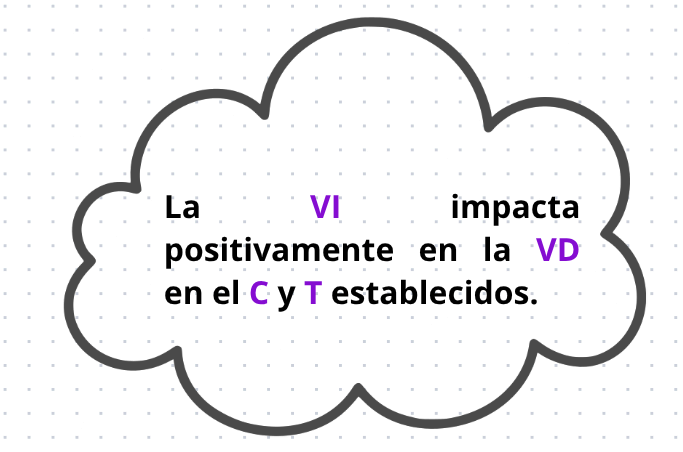
\includegraphics[width=7.0 cm]{src/imgs/hipótesis.png}

        \vspace{0.1cm}
        % \small EN CASO DE SER BAJO ELABORACIÓN PROPIA, NO HACE FALTA AGREGAR LA NOTA
    \end{figure}

    \begin{figure}[H]
        \centering
        %\isPreprints{\centering}{} % Only used for preprints
        \caption{Relación Inversa hasta la Hipótesis
        \label{fig-relacion-inversa-hipótesis}}    
                
        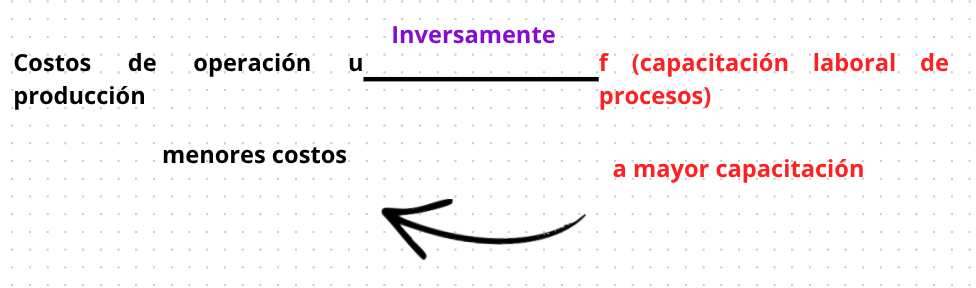
\includegraphics[width=11.0 cm]{src/imgs/relacion-inversa-hipotesis.png}

        \vspace{0.1cm}
        % \small EN CASO DE SER BAJO ELABORACIÓN PROPIA, NO HACE FALTA AGREGAR LA NOTA
    \end{figure}

\section{Hipótesis General}
    \begin{sectext}
        Lorem ipsum dolor sit amet consectetur adipisicing elit.
    \end{sectext}

\section{Hipótesis Específicas}
    \begin{sectext}
        \begin{itemize}
            \item Lorem ipsum dolor sit amet consectetur adipisicing elit.
            \item Lorem ipsum dolor sit amet consectetur adipisicing elit.
        \end{itemize}
    \end{sectext}

% -- SÉPTIMO CAPÍTULO --
% OPERACIONALIZACIÓN DE VARIABLES
\chapter{Operacionalización de Variables}
En una investigación científica, las variables son los elementos que permiten medir u observar los conceptos u fenómenos que estamos estudiando en una investigación. De manera exacta, podemos definir a una variable como cualquier característica que puede ser \textbf{medida, observar, manipular u controlar} en una experimentación u observación.

    \begin{figure}[H]
        \centering
        %\isPreprints{\centering}{} % Only used for preprints
        \caption{Tipos y características de una variable
        \label{fig-tipos-caracteristicas-variables}}    
                
        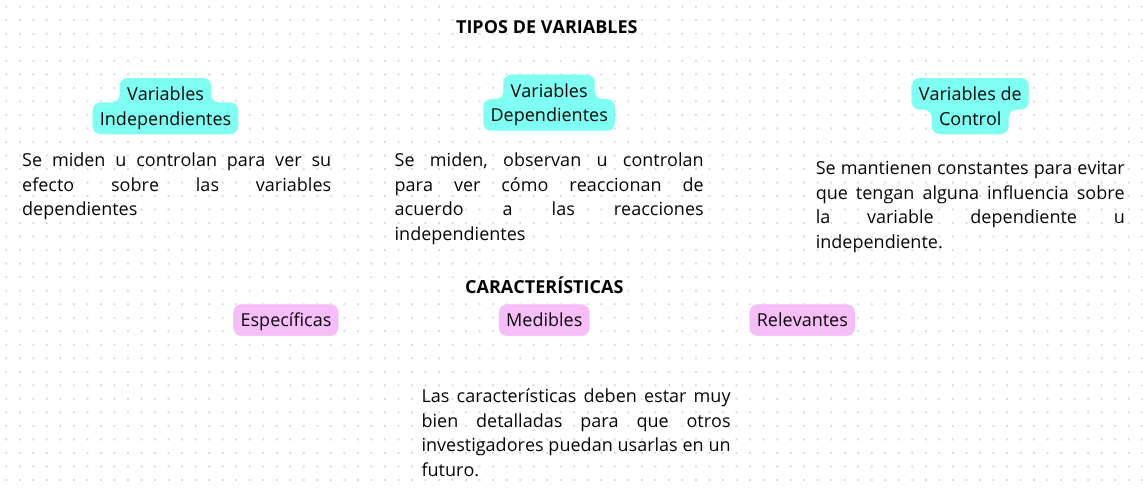
\includegraphics[width=10.0 cm]{src/imgs/tipos-variables.png}

        \vspace{0.1cm}
        % \small EN CASO DE SER BAJO ELABORACIÓN PROPIA, NO HACE FALTA AGREGAR LA NOTA
    \end{figure}

    \begin{figure}[H]
        \centering
        %\isPreprints{\centering}{} % Only used for preprints
        \caption{Ejemplo 1 - de Operacionalización de variables
        \label{fig-relacion-inversa-hipótesis}}    
                
        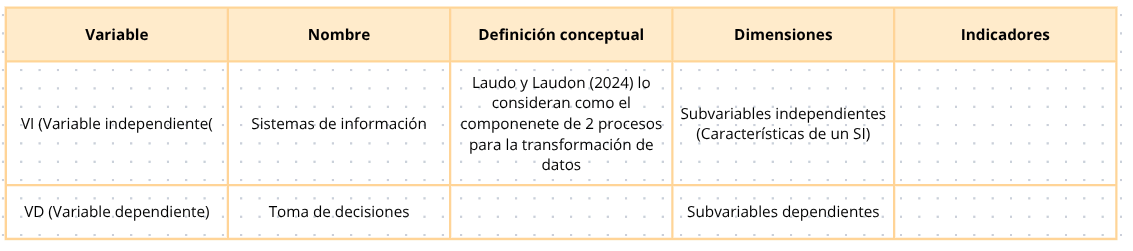
\includegraphics[width=10.0 cm]{src/imgs/operacionalizacion-variables-1.png}

        \vspace{0.1cm}
        % \small EN CASO DE SER BAJO ELABORACIÓN PROPIA, NO HACE FALTA AGREGAR LA NOTA
    \end{figure}

        \begin{figure}[H]
        \centering
        %\isPreprints{\centering}{} % Only used for preprints
        \caption{Ejemplo 2 - de Operacionalización de variables
        \label{fig-relacion-inversa-hipótesis}}    
                
        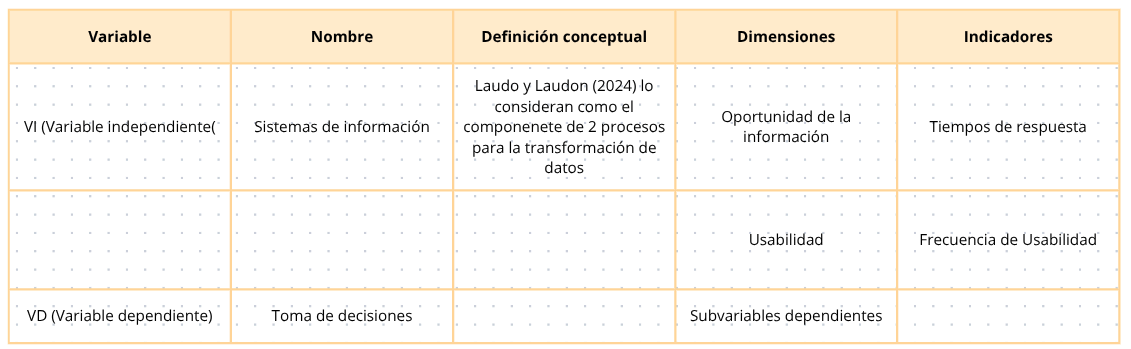
\includegraphics[width=10.0 cm]{src/imgs/operacionalizacion-variables-2.png}

        \vspace{0.1cm}
        % \small EN CASO DE SER BAJO ELABORACIÓN PROPIA, NO HACE FALTA AGREGAR LA NOTA
    \end{figure}

La definición conceptual a preferencia debe venir de teóricos (en lugar de solo autores de investigaciones).
Las dimensiones e indicadores debe salir de la teoría (De allí saldrá todo, puedes encontrarlo en otros lugares, pero a preferencia). En algunos casos también se utiliza la definición operacional. Esto será su valor matemático o algo así.

Ejemplo:
\begin{itemize}
    \item \textbf{Rentabilidad:}
    \begin{itemize}
        \item \textbf{De manera conceptual:} Es la utilidad u gannacia que tiene una empresa respecto a sus operaciones
        \item \textbf{De manera operacional:} Es la diferencia entre los ingresos  y egresos (gastos), siendo su fórmula: I - E
    \end{itemize}
\end{itemize}


% -- OCTAVO CAPÍTULO --
% METODOLOGÍA DE LA INVESTIGACIÓN
\chapter{Metodología de la Investigación}
\section{Tipo de Investigación}
    \begin{sectext}

        El tipo de investigación enmarca la idea del qué hacer y qué información necesito para lograr ese objetivo. Cada tipo de investigación conlleva una secuencia estructurada de fases y operaciones. Según \textcite{carrasco_dias_metodologia_2005}, existen 4 tipos de investigación: Investigación básica, donde se busca ampliar el conocimiento científico existente acerca de una realidad, el objetivo de este tipo de investigaciones recae sobre las teorías científicas; Investigación Aplicada, donde se buscan resultados prácticos e inmediatos por medio de actuar, transformar o modificar una parte de la realidad en estudio; Investigación Sustantiva, donde se busca responder a interrogantes concretas en favor de la consolidación de las teorías científicas y la aplicación de las investigaciones aplicadas y tecnológicas; por último, la Investigación Tecnológica busca perfeccionar u manipular un sector de la realidad en estudio mediante la aplicación de nuevos sistemas, modelos u técnicas.
        
        El presente trabajo se enmarca en el tipo de investigación tecnológica debido al objetivo central de realizar una invención tecnológica...
    \end{sectext}

\section{Nivel de la Investigación}
    \begin{sectext}
        El nivel de la investigación establece la profundidad que tendrá un estudio respecto a la problemática identificada. Según \textcite{carrasco_dias_metodologia_2005}, los niveles de investigación representan el orden secuencial y coherente que deben tener las investigaciones; se catalogan 4 tipos: preliminares o exploratorios, donde se establecen las primeras ideas y conceptos de la realidad a investigar; descriptivos, donde establecemos de manera robusta las propiedades, características, objetos, cualidades, rasgos u fenómenos de la realidad a estudiar; explicativos o causales, donde establecemos las causas u factores que dan origen a las circunstancias y naturaleza del fenómeno en estudio; y experimentales, en el cual se establece un nuevo paradigma, sistema, modelo u tratamiento para intentar corregir la situación problemática de la realidad en estudio.
        
        El presente trabajo se enmarca en el nivel de investigación de tipo experimental debido a que se busca entender cómo un nuevo sistema...
    \end{sectext}

% -- NOVENO CAPÍTULO --
% CRONOGRAMA
\chapter{Cronograma}
    \begin{table}[H]
        \caption{Cronograma de actividades estructurado en meses}
        \label{tab:cronograma}
        \begin{tabularx}{\textwidth}{X *{8}{c}}
            \toprule
            \textbf{DETALLES DE ACTIVIDADES} & \multicolumn{8}{c}{\textbf{TIEMPO EN MESES}} \\
            \cmidrule(lr){2-9}
            & \textbf{1°} & \textbf{2°} & \textbf{3°} & \textbf{4°} & \textbf{5°} & \textbf{6°} & \textbf{7°} & \textbf{8°} \\
            \midrule
            Formulación del Proyecto de Investigación. & X &   &   &   &   &   &   &   \\
            \addlinespace

            Elaboración del Proyecto & X & X &   &   &   &   &   &   \\
            \addlinespace

            Revisión de bibliografía y antecedentes. &   & X & X &   &   &   &   &   \\
            \addlinespace

            Presentación del Proyecto de investigación &   &   & X &   &   &   &   &   \\
            \addlinespace

            Inscripción del Proyecto de Investigación &   &   & X &   &   &   &   &   \\
            \addlinespace

            Selección y ordenamiento del cuerpo técnico y científico del problema de estudio. & X & X & X &   &   &   &   &   \\
            \addlinespace

            Preparación y elaboración de los instrumentos. &   &   &   & X &   &   &   &   \\
            \addlinespace

            Aplicación y recolección de datos. &   &   &   &   & X & X &   &   \\
            \addlinespace

            Análisis estadístico de los resultados. &   &   &   &   &   & X &   &   \\
            \addlinespace

            Interpretación de los resultados &   &   &   &   &   &   & X &   \\
            \addlinespace

            Elaboración de conclusiones &   &   &   &   &   &   & X &   \\
            \addlinespace

            Presentación del informe &   &   &   &   &   &   &   & X \\
            \addlinespace

            Evaluación y mejoramiento & X & X & X & X & X & X & X & X \\
            \bottomrule
        \end{tabularx}
    \end{table}

% -- DÉCIMO CAPÍTULO --
% PRESUPUESTO
\chapter{Presupuesto}

\begin{table}[H]
    \centering
    \caption{Presupuesto estimado para el desarrollo del plan de tesis}
    \label{tab:presupuesto}
    \begin{tabularx}{\textwidth}{X r}
        \toprule
        \textbf{Ítem / Rubro} & \textbf{Costo (S/.)} \\
        \midrule
        \multicolumn{2}{l}{\textbf{I. Maquinarias y Equipos}} \\
        \quad Laptop & 4,000.00 \\
        \quad Impresora & 1,450.00 \\
        \quad Memoria USB & 50.00 \\
        \addlinespace[0.5em]

        \multicolumn{2}{l}{\textbf{II. Recursos Humanos}} \\
        \quad Servicios Profesionales & 18,000.00 \\
        \quad Asesoría Especializada & 5,000.00 \\
        \addlinespace[0.5em]

        \multicolumn{2}{l}{\textbf{III. Materiales y Servicios de Oficina}} \\
        \quad Útiles diversos e insumos & 2,500.00 \\
        \addlinespace[0.5em]

        \multicolumn{2}{l}{\textbf{IV. Imprevistos}} \\
        \quad Contingencias operativas & 5,920.00 \\
        \midrule[\heavyrulewidth]
        \textbf{TOTAL GENERAL} & \textbf{S/. 36,920.00} \\
        \bottomrule
    \end{tabularx}
\end{table}

\chapter{Referencias Bibliográficas}
\printbibliography[heading=none]

% -- REFERENCIAS --
\addcontentsline{toc}{chapter}{REFERENCES}

% \chapter{Apéndices}
% \chapter{Anexos}
\end{document}